\pagebreak
\subsection{Mechanical Design} \label{Mechanical_Design}
\label{sec:mechanical-design}

The experiment consisted of two rectangular boxes, one stacked next to the other, shown in Figure \ref{dimensions}. The higher but narrower box (CAC box) allocated the heaviest element, the CAC. The main box (AAC box) contained the pneumatic system with six sampling bags and the central command unit: The Brain. The Brain contained the general Electronic box (EB) as well as the pneumatic sampling system.

The two-box design allowed ease of access and manipulation of both the CAC and AAC subsystems. In addition, the AAC sampling system is designed to be re-usable for future handover to the FMI, as such, it can be mounted on any standard balloon flight without having to introduce major design changes. The experiment would only require its own batteries as a power unit. In order to help balance the AAC box center of mass, they would be allocated in the corner opposite to the Brain, see Figure \ref{battery_distribution}. This also maintains the space for 6 bags inside the AAC box.

\begin{figure}[H]
    \centering
    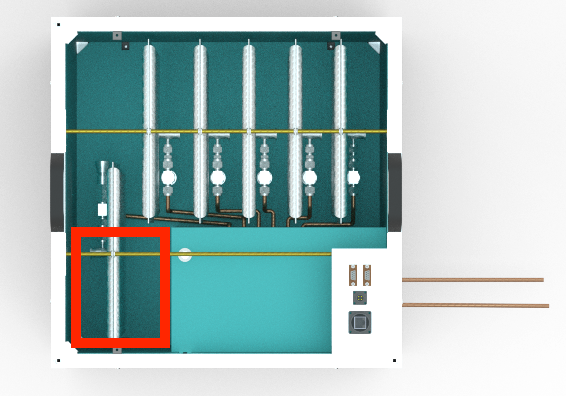
\includegraphics[width=0.8\textwidth]{4-experiment-design/img/Mechanical/Figure_15.png}
    \caption{Layout Including a Battery (in Red).}
    \label{battery_distribution}
\end{figure}

\pagebreak
Since the CAC was the heaviest component in the whole experiment its positioning and orientation inside the gondola will directly affect the stress analysis of the structure. In the worst case scenario, without a proper study of the aforesaid interface, shear in the screws could be produced after a violent landing stress or unexpected shaking. The larger the distance to the fixed points, the bigger the momentum produced by the component. For this reason, the CAC box was securely attached to the AAC box by means of six anchor points with four screws each. This fixing interface can be seen in red in Figure \ref{dimensions} to help the fast recovery. Taking into account also the two extra anchor points to the gondola, the fast recovery of CAC then only required unscrewing $16$ screws and unplugging a D-Sub connector.

 \begin{figure}[H]
     \centering
     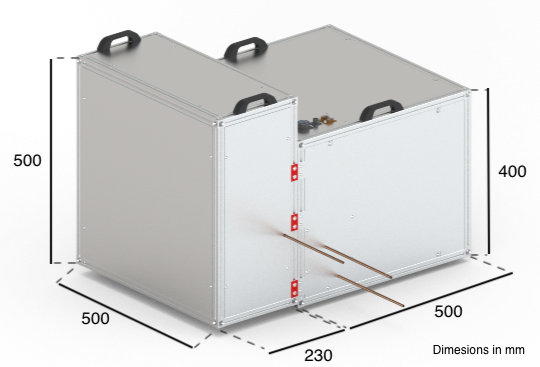
\includegraphics[width=0.9\textwidth]{4-experiment-design/img/Mechanical/Figure_14.png}
     \caption{General Dimensions of the Experiment.}
     \label{dimensions}
\end{figure}



The main mechanical characteristics of the experiment are summarized in Table \ref{table:experiment-summary}, where the values are based on the reference axis shown in Figure \ref{COG}. The Center Of Gravity for the whole experiment was determined to be located just on the plate of the third level of the Brain, which coincides with the location of the electronics PCB. This outcome was quite advantageous in terms of stability for one of the most sensitive subsystems of the experiment in terms of shakes and loads. 

\begin{table}[H]
\noindent\makebox[\columnwidth]{%
\scalebox{0.8}{
\begin{tabular}{c|c|c|c|}
\cline{2-4}
 & CAC & AAC & TOTAL \\ \hline
\multicolumn{1}{|c|}{Experiment mass {[}kg{]}} & $12.08$ & $12.37$ & $24.45$ \\ \hline
\multicolumn{1}{|c|}{Experiment dimensions {[}m{]}} & $0.23\times0.5\times0.5$ & $0.5\times0.5\times0.4$ & $0.73\times0.5\times0.5$ \\ \hline
\multicolumn{1}{|c|}{Experiment footprint area {[}m^2{]}} & $0.115$ & $0.25$ & $0.365$ \\ \hline
\multicolumn{1}{|c|}{Experiment volume {[}m^3{]}} & $0.0575$ & $0.1$ & $0.1575$ \\ \hline
\multicolumn{1}{|c|}{Experiment expected COG position} & \begin{tabular}[c]{@{}l@{}}$X=23.51\ cm$\\ $Y=10\ cm$\\ $Z=22.57\ cm$ \end{tabular}  & \begin{tabular}[c]{@{}l@{}} $X=29.04\ cm$\\ $Y=16.63\ cm$\\  $Z=16.2\ cm$ \end{tabular} &\begin{tabular}[c]{@{}l@{}} $X=26.31\ cm$\\ $Y=24.99\ cm$\\  $Z=19.35\ cm$  \end{tabular} \\ \hline
\end{tabular}}}
\caption{Experiment Summary Table.}
\label{table:experiment-summary}
\end{table}


 \begin{figure}[H]
     \centering
     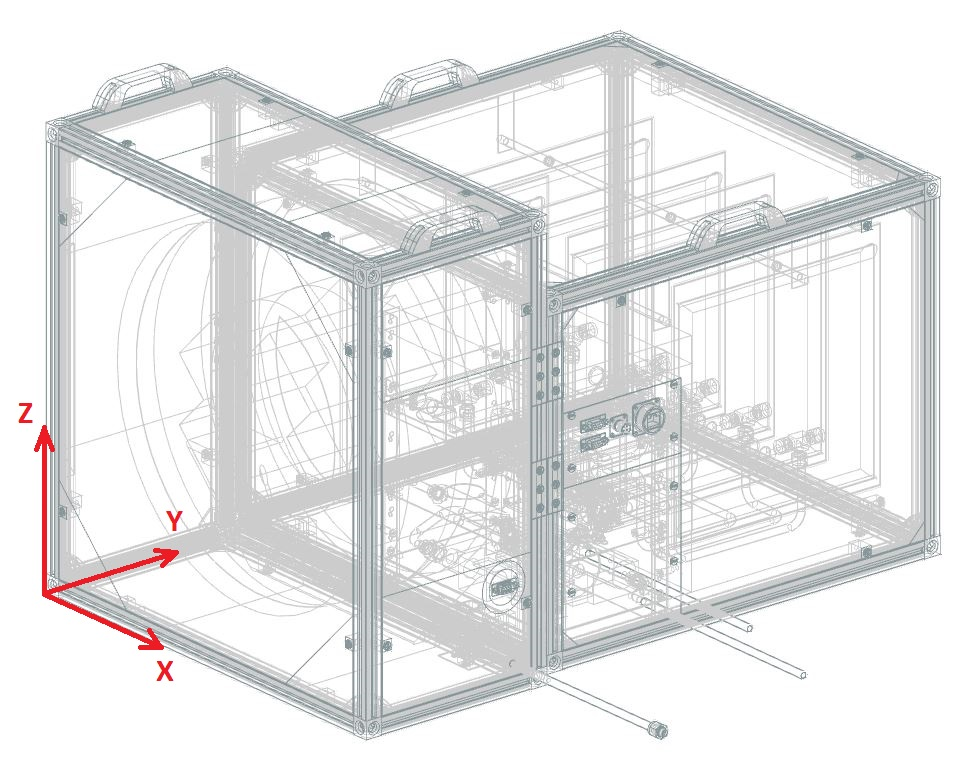
\includegraphics[width=0.45\textwidth]{4-experiment-design/img/Mechanical/COG.jpg}
     \caption{Reference Axis for the Total Center of Gravity.}
     \label{COG}
\end{figure}

\pagebreak
\subsubsection{Structure}
\label{sec:4.4.1}

The main purpose of the experiment box structure was to provide overall mechanical integrity and maintain the system geometry. It was able to carry the loads of all the phases of the flight and ensure that all the components and subsystems could withstand them. Test 9 in Table \ref{tab:vibration-test} helped to confirm the frame could withstand these vibrations.

Moreover, other considerations such as electrical and, especially, thermal conductivity were also a concern since the experiment flown up to $25\ km$ in the Polar Circle and many critical subsystems had tight operative ranges values.

 \begin{figure}[H]
     \centering
     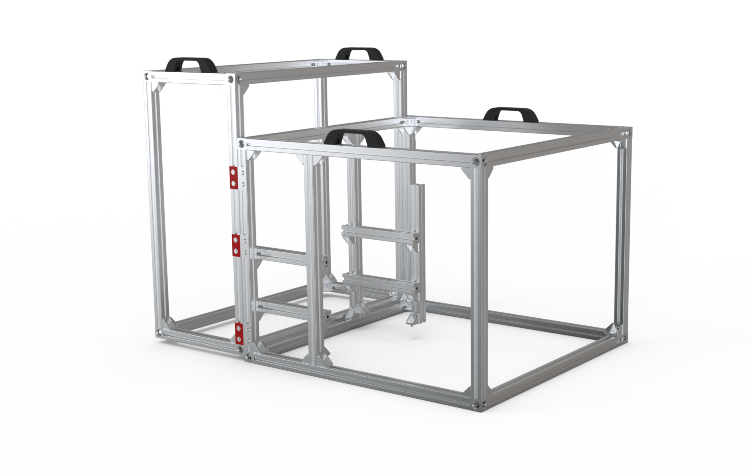
\includegraphics[width=0.8\textwidth]{4-experiment-design/img/Mechanical/structure.png}
     \caption{Structure Overview.}
     \label{fig:structure}
\end{figure}

For this purpose, two boxes built with straight frames were chosen as the best option as shown in Figure \ref{fig:structure}. The frame of these boxes were strut profiles made of aluminum, with a characteristic cross-section of $20\times20\ mm$, and with $M6$ thread at each side. The rails allowed an easy interface between bars and other elements. In turn, these profiles were joined together in each corner with aluminum cubic connectors of $20\times20\ mm$ (see Figure \ref{fig:corner_cube}) and $M6\times16$ bolts aligned with the bars axis. At the same time, these nodes were reinforced by three $20/20$ brackets (see Figure \ref{fig:corner_bracket}), each was fixed to the frames with $M4\times8$ bolts and the corresponding $M4$ T-nut. All these components were manufactured by Bosch Rexroth.

\bigskip
\begin{figure}[H]
    \noindent\makebox[\textwidth]{%
    \begin{subfigure}{.35\textwidth}
        \centering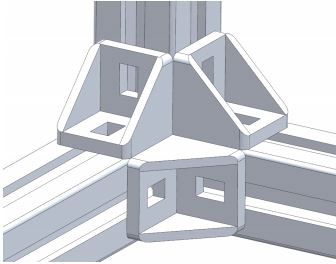
\includegraphics[width=1\textwidth]{4-experiment-design/img/Mechanical/corner_brackets.jpg}
        \caption{Brackets Reinforcement.}
        \label{fig:corner_bracket}
    \end{subfigure}
    \hspace{1cm}
    \begin{subfigure}{.35\textwidth}
        \centering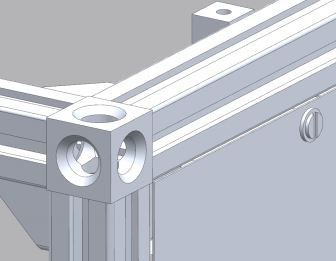
\includegraphics[width=1\textwidth] {4-experiment-design/img/Mechanical/corner_cube.jpg}
        \caption{Cubic Connector.}
        \label{fig:corner_cube}
    \end{subfigure}}
    \caption{Strut Profiles Connections.}
    \label{fig:profile_connection}
\end{figure}

\bigskip
Table \ref{table:profile_momentum} shows the main mechanical properties of the Bosch Rexroth $20/20$ strut profiles used in the structure. For further details see Table \ref{table:profile_material}.


\begin{longtable}{|m{0.2\textwidth}|m{0.14\textwidth}|m{0.25\textwidth}|m{0.3\textwidth}|}
\hline
\textbf{Section surface} & \textbf{Mass} & \textbf{Moment of Inertia ($I_x = I_y$)} & \textbf{Moment of resistance ($W_x = W_y$)} \\ \hline 
$1.6\ cm^2$ & $0.4\ kg/m$ & $0.7\ cm^4$ & $0.7\ cm^3$ \\ \hline

\caption{Intrinsic Characteristics of the Strut Profiles.}
\label{table:profile_momentum}
\end{longtable}

\smallskip

\subsubsection{Walls and Protections}
\label{sec:4.4.2}

Since the experiment was placed close to the outside of the gondola, it was very exposed to both external elements impacts and also possible broken parts from other experiments in the gondola due to unexpected rapid movements, and a probable hard landing impact. Therefore, the experiment box was shielded with removable aluminum walls along with a thick layer of Styrofoam attached to each wall. This thickness varied from two to three centimeters in the AAC box, and five centimeters to protect the AirCore. Besides protection, the thickness of the styrofoam was also motivated by thermal control issues.
% which is explained more in detail in Section \ref{sec:4.6.6}.

To mount the experiment a combination of three different elements were used, as shown in Figure \ref{fig:wall_attach}. The walls were screwed to the Variofix blocks by means of $M4\times8$ bolts. In between the aluminum walls and the bolts, a $M4$ retainer ring was placed to improve the fixation of each spot. Eight fixation points for each wall were considered sufficient to keep the experiment safe from any impact.

The styrofoam sheets were attached to the aluminum walls with double sided tape.

Tables \ref{table:wall_aluminum} and \ref{table:wall_styrofoam} show the main properties of the materials used to build the walls of the boxes.

 \begin{figure}[H]
     \centering
     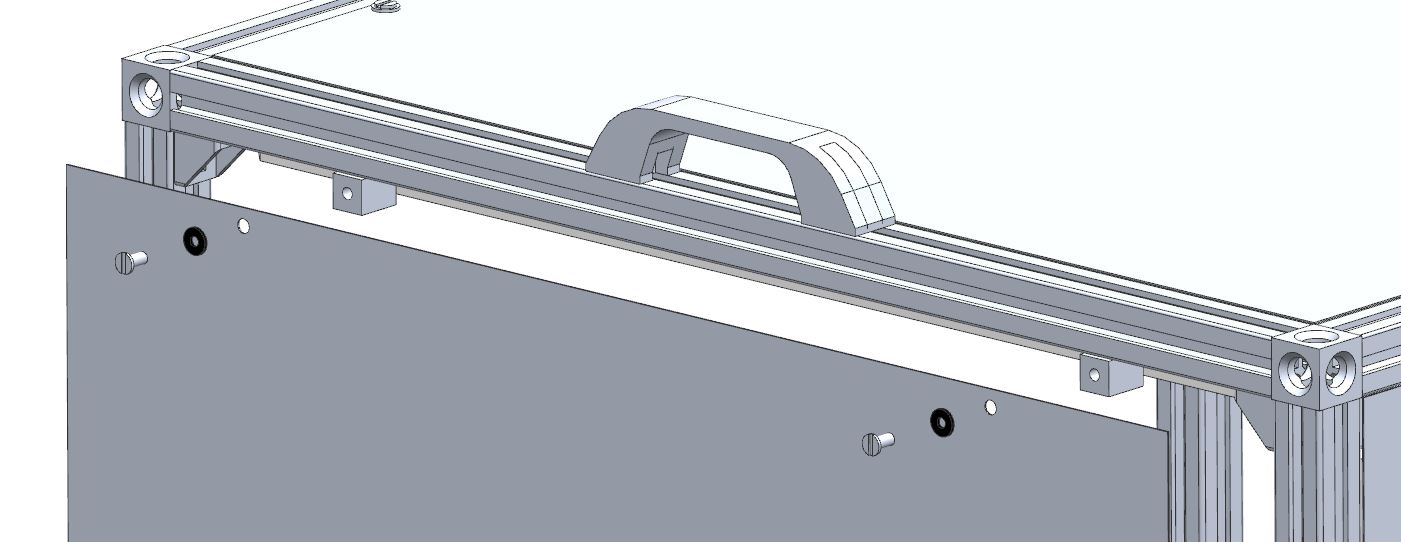
\includegraphics[width=0.5\textwidth]{4-experiment-design/img/Mechanical/wall_attachment.jpg}
     \caption{Exploit View of the Attachment of the Walls.}
     \label{fig:wall_attach}
\end{figure}

\subsubsection{CAC Box}

The CAC subsystem was designed to fit a $300$ m stainless steel coiled tube, a solenoid valve provided by SMC controlling it, tube fittings manufactured by Swagelok, an air filter and three temperature sensors. A schematic of this subsystem can be seen in Figure \ref{fig:CAC-schematic}. The CAC consisted of a combination of a $200$ m coiled tube of $1/8$ inches diameter and a $100$ m coiled tube of $1/4$ inches diameter. The outlet of the CAC was sealed with a quick connector provided by FMI. The inlet was sealed the same way but it could be opened by another interface plugged into the quick connector. A custom made filter by FMI was placed between this orifice and the solenoid valve. The filter contained magnesium perchlorate powder with stone wool at both ends of the tube. It ensured that no moisture entered the coil during any testing or sampling. A piece of stainless steel tube, manufactured by Silcotek, was attached to the solenoid valve that goes outside the box, thus having a direct outside outlet and inlet for the whole CAC system, as seen in Figure \ref{fig:CAC-cad-model}.

A D-sub cable was used to connect the electrical components to the control unit in the AAC box. Both boxes had their own D-sub connector, which was located on one of the box's walls.

% mechanical issues and gondola constraints 

\begin{figure}[H]
    \centering
    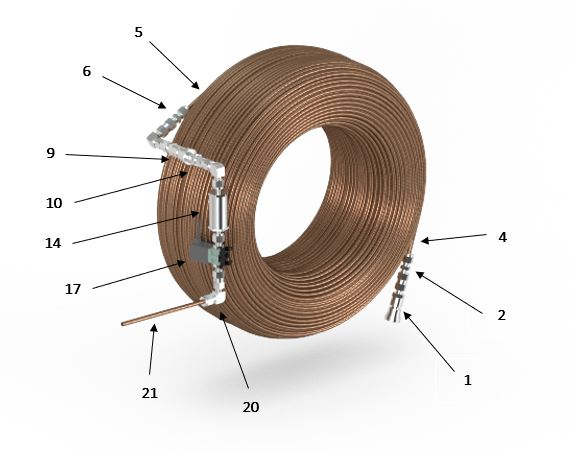
\includegraphics[width=0.6\textwidth]{4-experiment-design/img/Mechanical/CAC_labels.jpg}
    \caption{3D Model of the Aircore and its pneumatic fittings. The Numbers Correspond to the main components in Figure. \ref{fig:CAC-schematic}.}
    \label{fig:CAC-cad-model}
\end{figure}

\begin{landscape}
\begin{figure}[H]
    \centering
    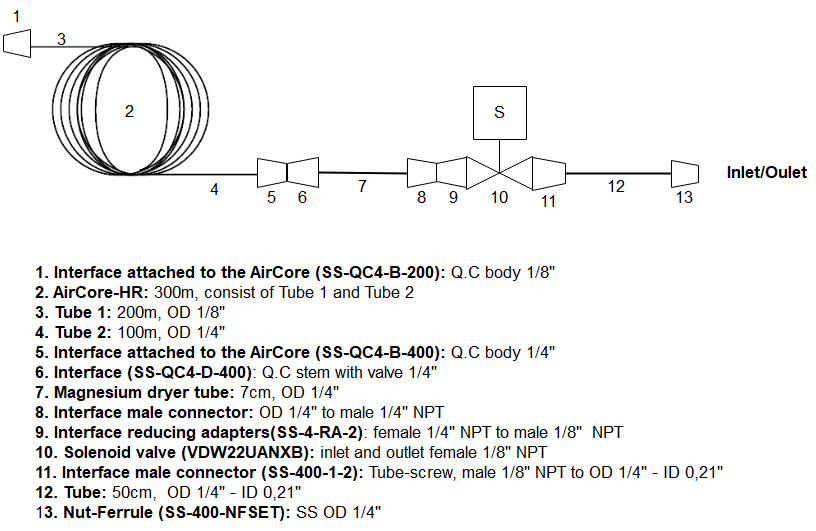
\includegraphics[width=1.3\textwidth]{4-experiment-design/img/Mechanical/CAC-schematic.PNG}
    \caption{Schematic of CAC.}
    \label{fig:CAC-schematic}
\end{figure}
\end{landscape}
\smallskip

\pagebreak
\subsubsection{AAC Box}\label{sec:aac-analysis}
The AAC box has been designed and manufactured to be as compact as possible. An analysis regarding the variation of the bags dimensions to different sampled volume, was made and is summarized in Appendix \ref{dimensions-bags}. From these results it was shown that the AAC subsystem was able to fit six $3\ L$ sampling bags, provided by RESTEK, together with The Brain that included the pneumatic system and the electronic box. Each bag had a dedicated valve in the Valve Center (VC) to allow emptying and filling processes as well as to close the bag when needed. The bags hung from a bar that was attached to the structure frame by two anchor points on the top. The distribution layout can be seen in Figures \ref{iso_aac} and \ref{lateral_aac}. To ensure a properly built pneumatic system with the minimal leakage risk, all tubes manufactured by Silcotek in the system were exclusively connected to tube fittings which were provided by Swagelok. 
 

\begin{figure}[H]
    \centering
    \begin{subfigure}[b]{0.47\textwidth}
        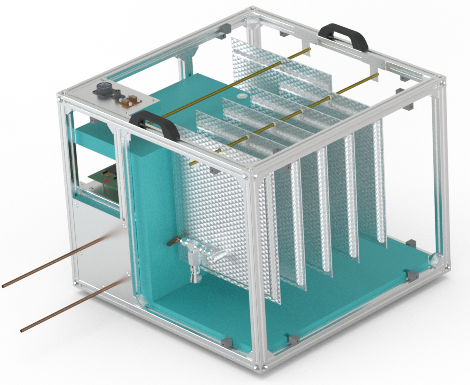
\includegraphics[width=\textwidth]{4-experiment-design/img/Mechanical/Figure_22a.png}
         \caption{Isometric View of the AAC Box.}
    \label{iso_aac}
    \end{subfigure}
    ~
    \begin{subfigure}[b]{0.47\textwidth}
        \centering
         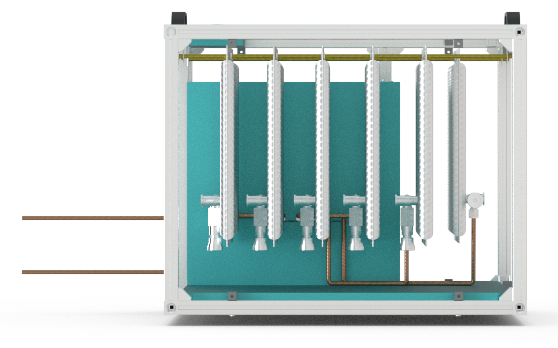
\includegraphics[width=\textwidth]{4-experiment-design/img/Mechanical/Figure_22b.png}
        \caption{Lateral View of the AAC Box.}
        \label{lateral_aac}
        \end{subfigure}
    \caption{Distribution Inside the AAC Box.}
    \label{fig:Distribution-AAC}
\end{figure}


The tubes going from the valve centre to the bags were sized as short as possible following science concerns regarding length.  


\pagebreak
\underline{The Brain}
\label{subsec:brain}

\smallskip
The Brain was an essential part of the experiment. It was a three-level structure containing both the pneumatic system and the electronics of the experiment, seen in Figure \ref{brain_isometric_open}. Its design made it compact enough to both allow a proper thermal control and to fit into the space left next to the sampling bags. It was placed in a corner of the AAC box. Therefore, The Brain took advantage of the vertical space inside the AAC box. It had three different levels: Level 1 - Pump, Level 2 - Valve Center, and Level 3 - Electronics.


\begin{figure}[H]
    \centering
    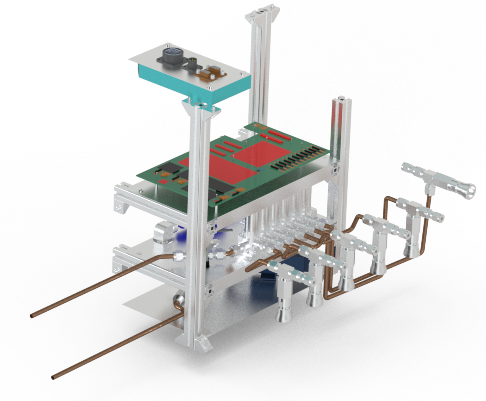
\includegraphics[width=0.7\textwidth]{4-experiment-design/img/Mechanical/Figure_23.png}
    \caption{Inside view of The Brain.}
    \label{brain_isometric_open}
\end{figure}

Level 1 of The Brain was lying on the base wall styrofoam. It contained the beginning of the pneumatic sampling system. The inlet tube passed through the wall and interfaced with the filter. From here the system continued through the pump provided by KNF, and to Level 2. The reason for having the pump in Level 1 was to have the minimum vibration transmitted to the other components. As explained in section \ref{subsec:vibration}, a piece of styrofoam was added between the pump and the level 1 plate to help mitigate its vibrations. The pump had two heaters on it that were used to regulate its temperature. %This can be seen as two black rectangular sheets underneath the pump in Figure \ref{level_1}.

The second level of The Brain was responsible for the distribution of the air to the selected sampling bag. From Level 1, the air passed through the airflow sensor and the static pressure sensor that allowed for monitoring the behavior of the system. The manifold with six solenoid valves, manufactured by SMC, was the main component. From here, the tubes were connected with the bags. A T-Union connection was used just before the bag valve. This interface allowed the pre-flight flushing of the tubes connecting with the valves as well as the post-flight analysis as explained previously. 

\smallskip
The flushing valve was responsible to ensure a proper flushing of the system before each sampling period. From the flushing valve, an outlet tube reached the outside environment. This can be seen in Figure \ref{level_2}.

The OBC and its external elements were allocated in the third level of The Brain. The PCB was fixed to the aluminum plate by means of 10 standoffs. As shown in Figure \ref{level_3}, it had a hole, as well as the level plate, to collect all the wires connecting with levels 1 and 2. This level had its own outside top wall which contained the electrical interfaces. The latter allowed the wall to be opened without having to remove all the sockets attached with screws and a female in the inside of the wall. The styrofoam shielding of The Brain had a hole on top to allow the temperature sensors wires to reach the inside of the AAC Box. 

A more detailed content of the components for each level is summarized in Appendix \ref{list-of-components-brain}.
\begin{figure}[H]
    \centering
    \begin{subfigure}[b]{0.3\textwidth}
    \centering
    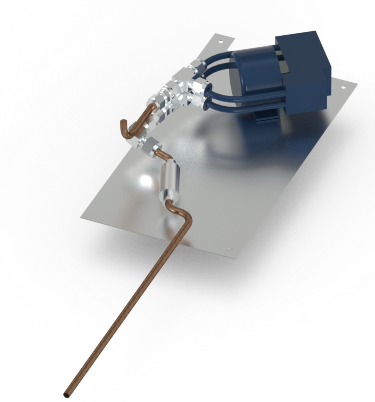
\includegraphics[width=\textwidth]{4-experiment-design/img/Mechanical/Figure_24a.png}
    \caption{Isometric View of Level 1.}
    \label{level_1}
    \end{subfigure}
    ~
    \begin{subfigure}[b]{0.3\textwidth}
    \centering
    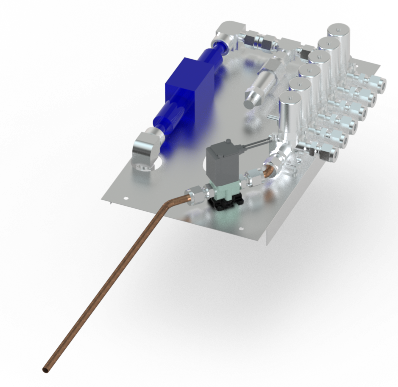
\includegraphics[width=\textwidth]{4-experiment-design/img/Mechanical/Figure_24b.png}
    \caption{Isometric View of Level 2.}
    \label{level_2}
    \end{subfigure}
    ~
    \begin{subfigure}[b]{0.3\textwidth}
    \centering
    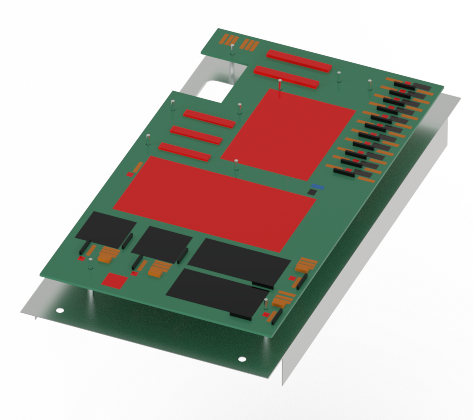
\includegraphics[width=0.8\textwidth]{4-experiment-design/img/Mechanical/Figure_24c.png}
    \caption{Isometric View of Level 3.}
    \label{level_3}
    \end{subfigure}
    \caption{Distribution in Each Level.}
    \label{fig:The-brain}
\end{figure}


This distribution allowed easy access to the PCB from the top and provides the physical desired separation between electronics and pneumatic circuit.


\smallskip
The structure of The Brain provided versatility in terms of implementation and construction. It was made out of strut profiles: four bars placed vertically and four bars placed horizontally. The railed bars allowed the possibility to fix all the pieces together and to provide the anchor points for the lateral and top styrofoam shield as well as to fix the whole unit to the box structure bars.

\smallskip
The bulk dimensions of The Brain were 260 mm long, 150mm wide and 290 mm high. If the shielding styrofoam walls were taken into account, the dimensions were 290 mm long, 180 mm wide and 300 mm high.
Therefore, accounting for the space the column bars took, each plate had a surface of 258 mm x 158 mm. The distance between levels was variable depending on the components dimensions. Level 1 had a height of 7 cm, Level 2 had a height of 9 cm and Level 3 had 8 cm to the top styrofoam shielding. The Brain with styrofoam shielding can be seen in Figure \ref{brain_isometric}.

\begin{figure}[H]
    \centering
    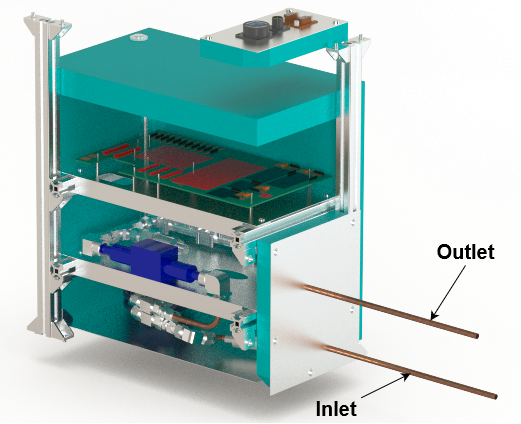
\includegraphics[width=0.6\textwidth]{4-experiment-design/img/Mechanical/Figure_25_0.png}
    \caption{Isometric View of The Brain.}
    \label{brain_isometric}
\end{figure}

\smallskip
In order to allocate the electrical interfaces required (E-Link, Power Supply and D-Sub Connectors) as well as to allow the tubes of the sampling system to reach the outside environment, the outside facing wall and the top wall were divided in two pieces each.  This made it easy to manipulate when having to open the box walls since the little pieces contained the interfaces and the tubes holes, were remained attached. The bottom piece covers Level 1 and 2 while the other, which contained the electrical connections, sat above Level 3. These pieces had the same layout as the main wall. 



\bigskip
\underline{Shielding and anchor points}

\smallskip
The most critical components in terms of required thermal control were inside The Brain. These were the pump and the valves. In order to provide a passive thermal shielding, 3 cm thick removable styrofoam walls were placed in the three walls (top, lateral, and rear) facing the interior of the AAC box, shown in Figure \ref{brain_isometric}. The lateral wall was fixed by means of four bolts that penetrated inside the styrofoam. The top wall was fixed to the rear wall and both were kept in place by means of a stoper. The larger lateral wall, where the tubes from the valves were, was divided in two pieces so it could be removed without having to disconnect the tubes. 

\smallskip
The Brain structure was integrated in the AAC box structure to provide the required stiffness to this element. 


\pagebreak
\subsubsection{Pneumatic Subsystem}
\label{sec:4.4.5}

In order to be able to collect separated samples of air, a pneumatic subsystem was developed and implemented. The schematics and components of this can be seen in Figure \ref{pneumatic_system}. The system was formed by almost $100$ components located inside The Brain and the AAC Box. 

In between these components, the same Sulfinert-treated stainless steel tubing as the ones used for the Inlet/Outlet pipes explained in Section \ref{subsec:pipes} were chosen. 

The schematic for the pneumatic system can be seen in Figure \ref{pneumatic_system}. The air was sucked from the outside through the inlet tube (No.1), the lower tube in Figure \ref{pneumatic_system_cad}, and it went through the filter (No.2) inside the pump (No.9). From here, and changing to Level 2, it passed through the airflow sensor (No.15), which allowed the airflow rate to be monitored. Thereafter the air passed through the static pressure sensor (No.20) before getting to the six station manifold (No.23). It was in here where the air was directed to the desired bag (No.36) thanks to its dedicated solenoid valve (No.30).

When flushing the pneumatic system before each sampling period, the flushing valve (No.27) was opened so that the outlet of the system was open and new air ran through the main part of the pneumatic system. 


\begin{figure}[H]
    \centering
   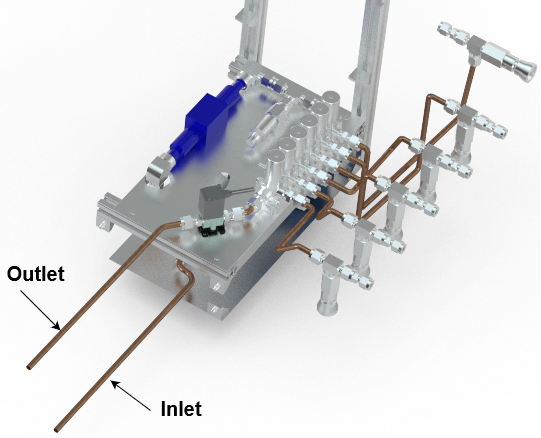
\includegraphics[width=0.8\textwidth]{4-experiment-design/img/Mechanical/Figure_26.png}
   \caption{Pneumatic System Top View.}
    \label{pneumatic_system_cad}
\end{figure}


\begin{landscape}
\begin{figure}
    \centering
    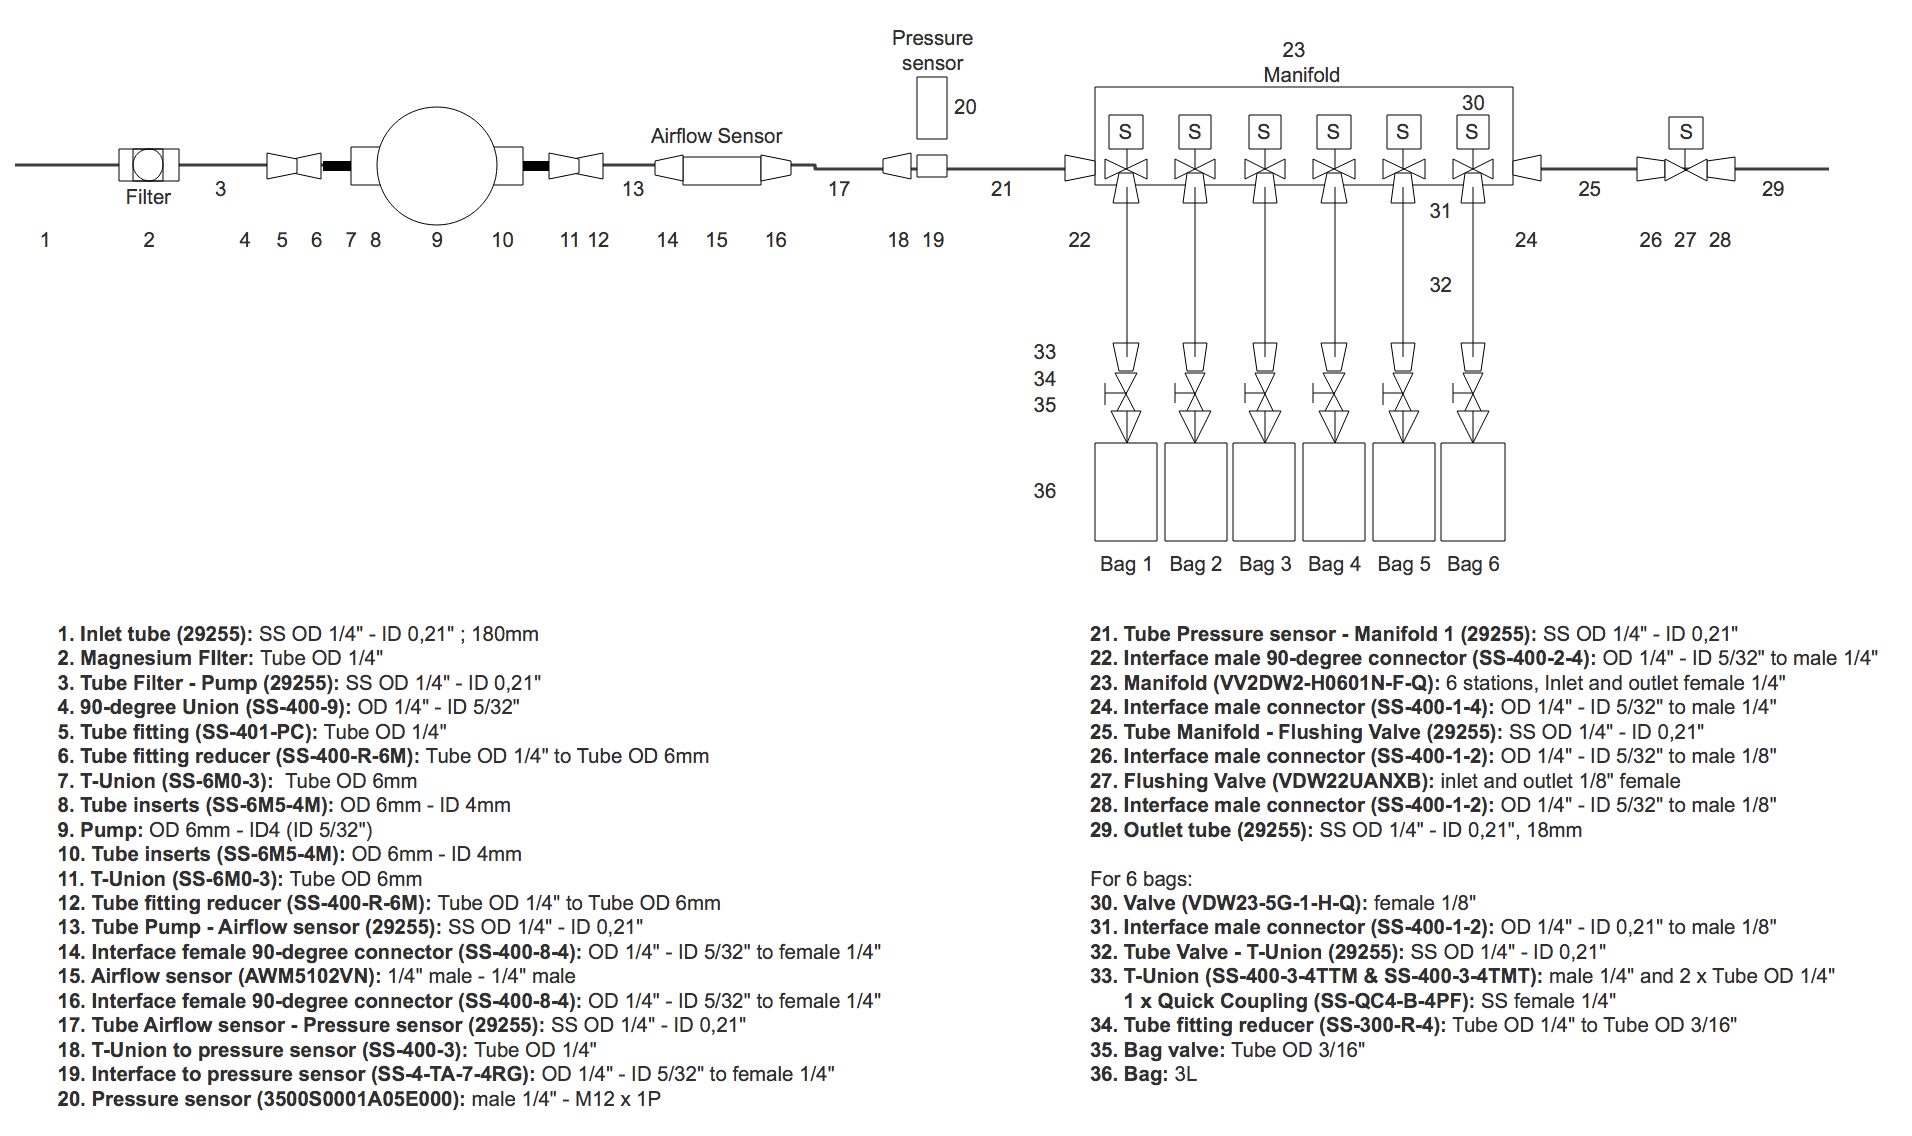
\includegraphics[width=1.45\textwidth,height=\textheight]{4-experiment-design/img/Mechanical/AAC_System.png}
    \caption{AAC Pneumatic System Diagram and Components.}
    \label{pneumatic_system}
\end{figure}
\end{landscape}

%\raggedbottom